\documentclass[12pt]{article}
\usepackage[table]{xcolor}
\usepackage{pdflscape}
\usepackage{graphicx}
\usepackage[hidelinks]{hyperref}
\usepackage[numbers]{natbib}
\usepackage{etoolbox}
\apptocmd{\thebibliography}{\raggedright}{}{}
\usepackage{setspace}
\usepackage{pdfpages}
\usepackage{svg}
\hypersetup{ colorlinks, citecolor=black,
	filecolor=black,
	linkcolor=black,
	urlcolor=blue,
	pdftitle={M.O.S.I.S Progress Report},
	pdfpagemode=FullScreen,
}
\usepackage[subpreambles=true]{standalone}
\usepackage{import}

\begin{document}
\pagenumbering{gobble}
\linespread{1.0}
\begin{titlepage}
	\begin{center}
		\large{University of Puerto Rico\\
			Mayagüez Campus\\
			\vspace{\baselineskip}
			Department of Electrical and Computer Engineering}\\
		\vspace{5\baselineskip}
		\Huge{\underline{M.O.S.I.S U.I 2.0 Progress Report}\\}
		\vspace{\baselineskip}
		\large by\\
		Fabio J. Matos Nieves\\
		Eduardo S. Miranda Figueroa\\
		\normalsize
		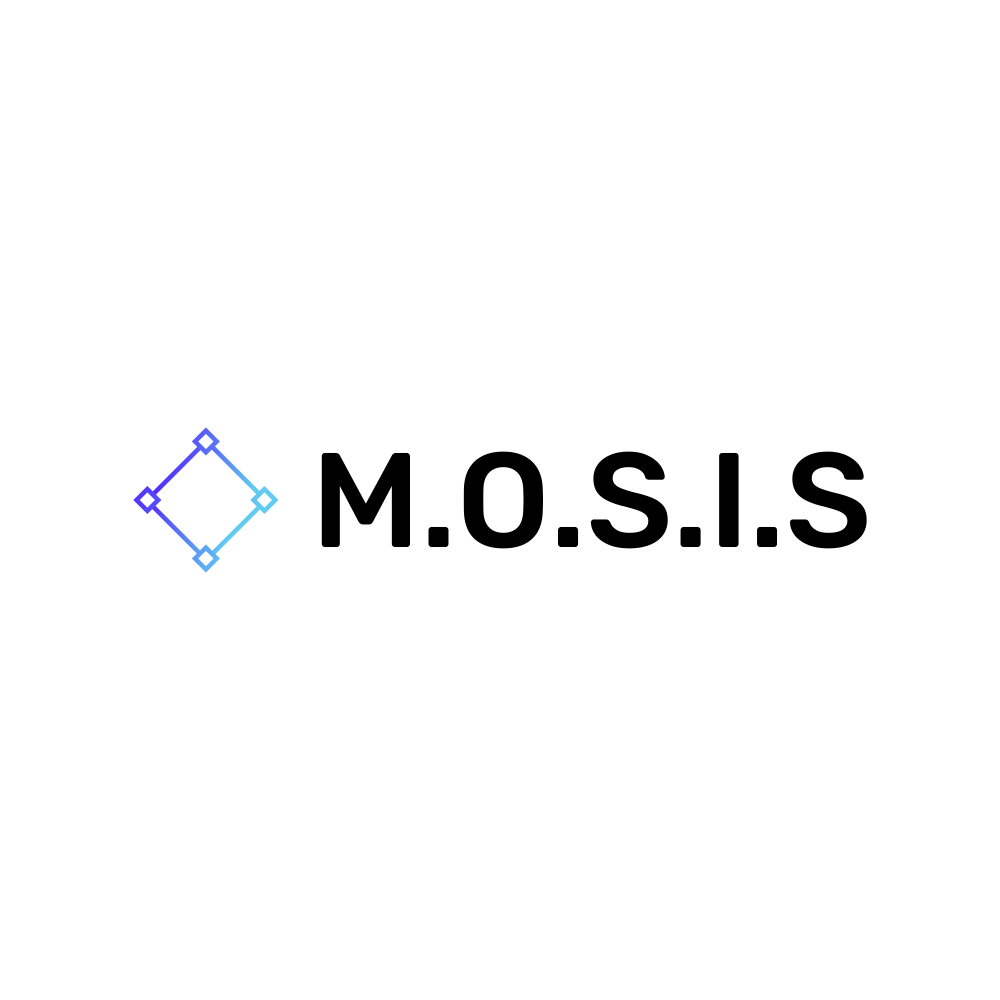
\includegraphics[scale=0.15]{../../M.O.S.I.S Logo/default.png}\\
		\vspace{4\baselineskip}
		\large
		For: Nayda Santiago\\
		Course: ICOM 5047, section 016\\
		Date: September 14, 2023\\
		\normalsize

	\end{center}
\end{titlepage}
\section*{Executive Summary (Fabio)}
\begin{spacing}{1.5}
\end{spacing}
\pagenumbering{roman}
\tableofcontents
\listoffigures
\newpage
\pagenumbering{arabic}
\begin{spacing}{1.2}
	\section{Introduction (Fabio)}
The fundamental problem with the UI currently employed on the M.O.S.I.S is a lack of design cohesion, missing and redundant features, constant crashing and lacks a formal way to store the data on the microscope. This problem has not fundamentally changed since the proposal. However, there has been one major objective change since then, that being that no longer will the preview of the cameras be at 1920x1080 resolution. Since reviewing the data sheet of the LCD display on the microscope, we have determined to have resolution 400x200 would be more appropriate since the resolution of the display is 800x480.\cite{5inchResistiveTouch} This allows the preview feed to be at the native aspect ratio of the display while allowing space for the sensor data. The following are the updated project objectives:
\begin{enumerate}
	\item Design a UI for the M.O.S.I.S project Raspberry Pi by November 27, 2023 to:
	      \begin{itemize}
		      \item Control the functions of the microscope, utilizes the onboard buttons, shows a live preview at 15 FPS at a downscaled resolution of 400x200
		      \item Display temperature sensors data with an accuracy of 3 significant digits
		      \item Display Ph sensor data with an accuracy of 3 significant digits
		      \item Display pressure sensor data with an accuracy of 3 significant digits.
		      \item Display dissolved oxygen sensor data with an accuracy of 3 significant digits
		      \item Display current local IP address
		      \item Choose the configuration file for the specific study to be done
		      \item Achieving a tenfold decrease in transition time in comparison to the existing user interface when switching through different windows in the user interface
	      \end{itemize}
	\item Adapt the currently existing hardware API, by November 27, 2023 to:
	      \begin{itemize}
		      \item Display the live feed from the cameras to the U.I
		      \item Parse the temperature, Ph, pressure and dissolved oxygen data string from the UART port
		      \item Run diagnostic sub-routines at application start
	      \end{itemize}
	\item By November 27, 2023, store data and metadata in a format that a researcher can browse through in a file browser, of which include:
	      \begin{itemize}
		      \item Left camera media
		      \item Right camera media
		      \item Shot type
		      \item Time stamp
		      \item Temperature
		      \item Ph
		      \item Pressure
		      \item Dissolved oxygen
	      \end{itemize}
\end{enumerate}
This progress report is organized as into the following parts:
% \begin{enumerate}
% 	\item Technical Progress:
% 	      \begin{enumerate}
% 		      \item Describes design alternatives
% 		      \item Analysis criteria for the design alternatives
% 		      \item Justifies choices made for the project
% 		      \item Presents and describes the system architecture
% 		      \item Design progress describing system components
% 		      \item Present basic technical diagrams (Detailed descriptions, calculations and diagrams will be in the appendix)
% 	      \end{enumerate}
% \end{enumerate}
\begin{enumerate}
	\item Technical Progress: Describes at a high level the design process for this project.
	\item Task Progress: Analyzes the current project state with projected schedule and update it accordingly
	\item Expenditure Analysis: Analyses current expenditures on components and personnel and summarizes expected remaining costs.
	\item Next Steps: Describes upcoming tasks
	\item Appendix: Contains detailed descriptions, calculations and diagrams of the design process
\end{enumerate}
	\section{Technical Progress (Fabio \& Eduardo)}
\subsection{Design Alternatives}
Since we are designing a user interface 3 main design platforms arise:
\begin{enumerate}
	\item Web-based
	\item Web-Native
	\item Native
\end{enumerate}
Web-based mean having a client server relationship within the system and having all interacting occurring within the browser.
Native is writing a user interface from scratch that executes on the native operating system.
Web-native is a hybrid approach that uses web technologies in a native platform.
\subsection{Analysis Criteria}
Since at its core, the M.O.S.I.S microscope is an embedded system the following limitations need to be taken into consideration:
\begin{itemize}
	\item Single Core
	\item Low CPU clock frequency
	\item ARM Architecture
	\item Limited system memory
	\item Raspberry Pi official library compatibility
\end{itemize}
With these restrictions in mind, the criteria used in our analysis are as follows:
\begin{itemize}
	\item Has to utilize Python
	\item Minimize CPU load
	\item Minimize Memory Usage
	\item Easily interfaces with existing hardware API functions
	\item Easily interfaces with on-board buttons
	\item Easily interfaces with the file system
	\item Can easily be backed up and be restored from a backup
\end{itemize}
\subsection{Design Justifications}
Based on the analysis criteria, we have chosen to create a native user interface in Python using PyQt6, a SQLite database and specific folder specific format.\cite{PyQt2023}\cite{SQLite2023} The reason why Python was chosen was simple, the official Raspberry Pi library that is used to access embedded peripherals only officially supports Python. There are bindings for other languages like Rust but they are not officially supported by the Raspberry Pi developers. In addition the existing camera API  is already written in Python. Secondly, the reasons why PyQt6 was chosen for our graphical user interface library were:
\begin{itemize}
	\item Qt is an established, open source, GUI library used across Linux
	\item Qt is much easier to modify the look and feel compared to other open source libraries such GTK
	\item Qt has a much more stable development cycle compared to GTK
	\item PyQt6 are open source Python binding for the Qt6 library that is originally written in C++
\end{itemize}
Thirdly, SQLite was chosen as our database engine because:
\begin{itemize}
	\item Due to the database being in a file rather than a server, it facilitates the process of backing up the database
	\item It is much less resource intensive than server based alternatives such as MongoDB and MariaDB
	\item The reduction in types simplifies and hastens query execution on embedded systems
	\item The reduction in types allows for the database to the compressed much more efficiently
\end{itemize}
\subsection{System Architecture and Interfaces}
The M.O.S.I.S microscope itself has 5 fundamental parts:
\begin{enumerate}
	\item Raspberry Pi
	\item Cameras
	\item Sensors
	\item Display
	\item Buttons
\end{enumerate}
The Raspberry Pi serves as main microcontroller that receives input from the cameras, sensors and buttons and presents it on the display.
The cameras are connected to the Pi via USB and have basic functionality as webcams but can be further configured in software using the SDK for the cameras. The sensors are configured and utilized by the onboard Tiva microcontroller and the Pi received the captured data via a UART port. The buttons utilize the GPIO interface on the Pi and are operated via interrupts. The display uses a HDMI interface to present the desktop environment of the Raspberry Pi real time operating system.\\
As for the UI, it is comprised of:
\begin{itemize}
	\item Front End User Interface
	\item Database
	\item Hardware API
	\item Folder Structure Generator
\end{itemize}
The front end user interface is presented on the Raspberry Pi display via the Raspberry Pi OS desktop environment. The database is the storage medium for all of the metadata captured by the microscope. Camera image paths, date and time stamp, shot type, illumination type, sensor data, camera ISO, shutter speed,aperture size and white balance will all be placed in the database and will serve as the permanent record for the microscope. The hardware API will serve as the interface between the sensors, the cameras and the solid state disk on the microscope to communicate with the operating system to control the camera functions, interacting with the sensors and writing media files to disk. The sensors will be interacted with via UART, the cameras will be manipulated using the library functions provided by the manufacturer, via the USB interface. The sensor and image data will manipulated in software and written to disk using operating system calls.
\subsection{System Modules}
M.O.S.I.S UI 2.0 can be divided into 4 modules:
\begin{itemize}
	\item Front End
	\item Database
	\item Hardware API
	\item Folder Structure Generator
\end{itemize}
The front end consists of all of the UI elements, i.e preview screen, study select, sensor calibration menus and camera control menus.\cite{UnifiedModelingLanguage}
The database module consists of the SQLite database and all statements to insert and select data.\cite{kelechavaSQLStandardISO2018}\cite{UnifiedModelingLanguage} The hardware API is the camera control and sensor hub, bi-directional, communication protocols. Finally, the folder structure generator is comprised of interfaces between the database and file system to generate the browsable folder structure and exporting the metadata from the database to a JSON file.\cite{JPEGJPEG}\cite{JSON}
\subsection{Technical Diagrams}
\begin{center}
	\begin{figure}[H]
		\centering
		\resizebox{!}{0.6\textheight}{
			\import{../Appendix/Design_Documentation/Use_Case_Diagram/Figures/}{use_case}
		}
		\caption*{M.O.S.I.S UI 2.0 Use Case Diagram}
	\end{figure}
	\begin{figure}[H]
		\resizebox{\textwidth}{0.4\textheight}{
			\import{../Appendix/System_Architecture_and_Interfaces/Software_Architecture/Figures}{system_architecture}
		}
		\caption*{M.O.S.I.S UI 2.0 Software Architecture}
	\end{figure}
\end{center}
	\section{Task Progress (Fabio)}
Upon further analysis, the original schedule was unfeasible since it calculated based on 100\% capacity which is unobtainable in the real world with inevitable delays and happenstance occurring constantly. Upon further consideration, we have adjusted the training load to be 25\% and the implementation load to be 50\%. The reason why the training load is 25\% is that upon starting the course, we have noticed that it takes on average 1.5 times the lesson length to complete a lesson, since we implement what was taught in the video in out own development environment. This helps solidify what was taught in the lesson but has the downside of both increasing training time and developer burn out, thus a 25\% work load was chosen to more accurately reflect how we proceed through the lessons of the PyQt6 course. The 50\% work load during product implementation was chosen to consider real life delays and happenstance but to also not underestimate developer speed and competence. Another side effect of choosing a 50\% work load is we achieve 13 days of lag between the final deadline which allows for a substantial amount of leeway for delays.\\
Up to this point we are progressing through the PyQt6 course at a albeit slow but steady pace. Mainly, we have finished the introduction and about one quarter of the widgets section, which is about 5\% complete of the course according to Udemy statistics.
	\section{Expenditure Analysis (Eduardo)}
The difference between the estimated and actual cost of the project are due to the equipment cost were calculated assuming the M.O.S.I.S microscope and laptops needed to be bought. They were bought and made beforehand. \\
\begin{table}[h]
    \centering
    \textbf{Estimated Cost}\\
    \begin{tabular}{||c | c||} 
     \hline
     \rowcolor{cyan!50}
     Category & Cost \\ [0.5ex] 
     \hline
     Human Resources & \$18,430.61\\ 
     \hline
     Equipment & \$7,961.98\\
     \hline
     Facility & \$1,410.00\\
     \hline
     Overhead Cost & \$13,901.01\\
     \hline
     \rowcolor{teal!50}
     Total Estimated Cost & \$41,703.03\\
     \hline
    \end{tabular}
    \caption {Total Estimated Cost of the Project}
    \label {table:1}
\textbf{Actual Cost}\\
    \begin{tabular}{||c | c||} 
     \hline
     \rowcolor{cyan!50}
     Category & Cost \\ [0.5ex] 
     \hline
     Human Resources & \$18,430.61\\ 
     \hline
     Equipment & \$29.98 \\
     \hline
     Facility & \$1,410.00\\
     \hline
     Overhead Cost & \$9,934.74\\
     \hline
     \rowcolor{teal!50}
     Total Actual Cost & \$29,804.22\\
     \hline
    \end{tabular}
    \caption {Total Actual Cost of the Project}
    \label {table:2}
\end{table}
The difference between the estimated cost and actual cost is \$11,900.81.
\textit{\$41,703.03 - \$29,804.22 = \$11,900.81}\\
	\section{Next Steps (Fabio)}
As for what needs to be done next, before the progress report presentation is due, we will finish the Udemy course on PyQt6, design the database schema for the M.O.S.I.S UI and create a mock-up for the UI. As for speeding up training, we will be culminating the course at ``Section 15: PyQT6.2 released with QtMultimedia \& QtWebEngine Modules'' and skipping sections 9,11,12,13 since that are irrelevant to our project objectives. After the mock-up is approved by the client, the front-end milestone can be implemented and completed by October fifteenth.
\end{spacing}
\addcontentsline{toc}{section}{Bibliographic References}
\printbibliography
\appendix
\section{Glossary (Fabio \& Eduardo)}
\begin{description}
	\item[UI] User Interface
	\item[GUI] Graphical User Interface
	\item[Open Source] Product that is free to modify, download and review
	\item[M.O.S.I.S] Marine Operated Stereoscopic Imaging System
	\item[FPS] Frames per Second
	\item[Pixel] Fundamental unit of an image, normally comprised of a red, green and blue elements
	\item[Resolution] Pixel dimension of an image
	\item[Downscale] Reduce the resolution of an image
	\item[Ph] Power of hydrogen, used to measure how acidic or basic a substance is
	\item[IP Address] Internet Protocol Address
	\item[Live feed] Constantly updating data stream
	\item[Sub-routine] Smaller part of a program, usually executes independently from the main process
	\item[Metadata] The data about data
        \item[Media] Video and Pictures
        \item[Lighting] The type of illumination on a subject
        \item[None] No LED illumination on the subject
        \item[Infrared] LEDs that emit 700nm to 1mm wavelength of light
        \item[Ultraviolet] LEDs that emit 100nm to 400nm wavelength of light
        \item[Visible Spectrum] LEDs that emit 380nm to 700nm wavelength of light
        \item[Shot Type] Single, burst, telescopic, time lapse and video photography
        \item[Single] A single image capture
        \item[Burst] Multiple images captured in succession
        \item[Telescopic] A burst capture where the camera zooms out before capturing a new image
        \item[Time Lapse] Images captured at a specified interval
        \item[Video] A sequence of images captured in succession at a specific FPS
        \item[Back End] Database management component
        \item[API] Application Programming Interface
        \item[Hardware] Physical components of a electronic device
        \item[Software] Instructions that are executed on hardware
        \item[Study Profile] Contains all parameters for lighting and shot type
        \item[Study Entry] A single, executed study profile
        \item[Stepper Motor] A type of motor that rotates in steps by changing the currently active phases
        \item[CPU] Central Processing Unit
\end{description}
\section{Requirements (Fabio \& Eduardo)}
\subsection{Domain Requirements}
\begin{itemize}
	\item The system-to-be must present the left and right camera feeds to the user.
	\item The system-to-be must present temperature, pH, dissolved oxygen, pressure, study status, and local IP address to the user.
	\item The system-to-be must have the means to switch between different study profiles
	\item The system-to-be must control the lighting on the microscope cameras according to the study profile.
	\item The system-to-be must control the shot type on the microscope cameras according to the study profile.
	\item The system-to-be must control the gain of the microscope cameras.
	\item The system-to-be must control the saturation of the microscope cameras.
	\item The system-to-be must control the shutter speed of the microscope cameras.
	\item The system-to-be must control the white balance of the microscope cameras.
	\item The system-to-be must call the calibration functions of the microscope sensors.
	\item The system-to-be must have a database that stores:
	      \begin{itemize}
		      \item Left Camera Media
		      \item Right Camera Media
		      \item Shot type
		      \item Modified ISO 8601 Date Stamp (yyyy-MM-ddTHHmm-ss.zzz)
		      \item Temperature
		      \item pH
		      \item Pressure
		      \item Dissolved Oxygen
		      \item Illumination Type
		      \item Gain
		      \item Saturation
		      \item Shutter Speed
		      \item White Balance
	      \end{itemize}
	\item The system-to-be must store the captured data into a browsable format.
	\item The system-to-be must use the on board buttons to control the functions of the microscope.
\end{itemize}
\subsection{Interface Requirements}
\begin{itemize}
	\item The system-to-be must present the feed from left and right cameras at downscaled 400x400 resolution at $1/3$ frames per second.
	\item The system-to-be must present: temperature, pH, pressure, dissolved oxygen, study status, gain, saturation and shutter speed, white balance and IP address.
	\item The system-to-be must update temperature, pH, pressure, dissolved oxygen and local IP address, study status, every two seconds due to the existing UART implementation.
	\item The system-to-be lighting enumeration contains:
	      \begin{itemize}
		      \item None
		      \item White
		      \item Ultraviolet
		      \item Red
	      \end{itemize}
	\item The system-to-be shot type enumeration contains:
	      \begin{itemize}
		      \item Single
		      \item Burst
		      \item Telescopic
		      \item Time Lapse
		      \item Video
	      \end{itemize}
	\item The system-to-be must initiate a capture with a single button.
	\item The system-to-be must shutdown the operating system safely using 1 button.
	\item The system-to-be must stop capture with a single button.
	\item The system-to-be must be able to navigate through the study profiles using only two buttons.
	\item The system-to-be must show the currently loaded study profiles using a single button.
	\item The system-to-be must store all files related to a single study entry in a single directory.
	\item The system-to-be must store a JSON file with all data and metadata from the study entry along in the same directory as the study entry.
	\item The system-to-be must control the focus of the cameras 5 focus step at a time using two buttons.
	\item The system-to-be must control the gain of the cameras using two buttons.
	\item The system-to-be must show all available camera gain values using a single button.
	\item The system-to-be must control the saturation of the cameras using two buttons.
	\item The system-to-be must show all available saturation values using a single button.
	\item The system-to-be must control the shutter speed of the cameras using two buttons.
	\item The system-to-be must show all available shutter speeds using a single button.
	\item The system-to-be must control the white balance of the cameras using two buttons.
	\item The system-to-be must show all available white balance using a single button.
\end{itemize}
\includepdf[pages=1-2]{../Appendix/Requirements/Figures/signed_requirements.pdf}
\includepdf[pages=3-4, width=1.5\textwidth]{../Appendix/Requirements/Figures/signed_requirements.pdf}
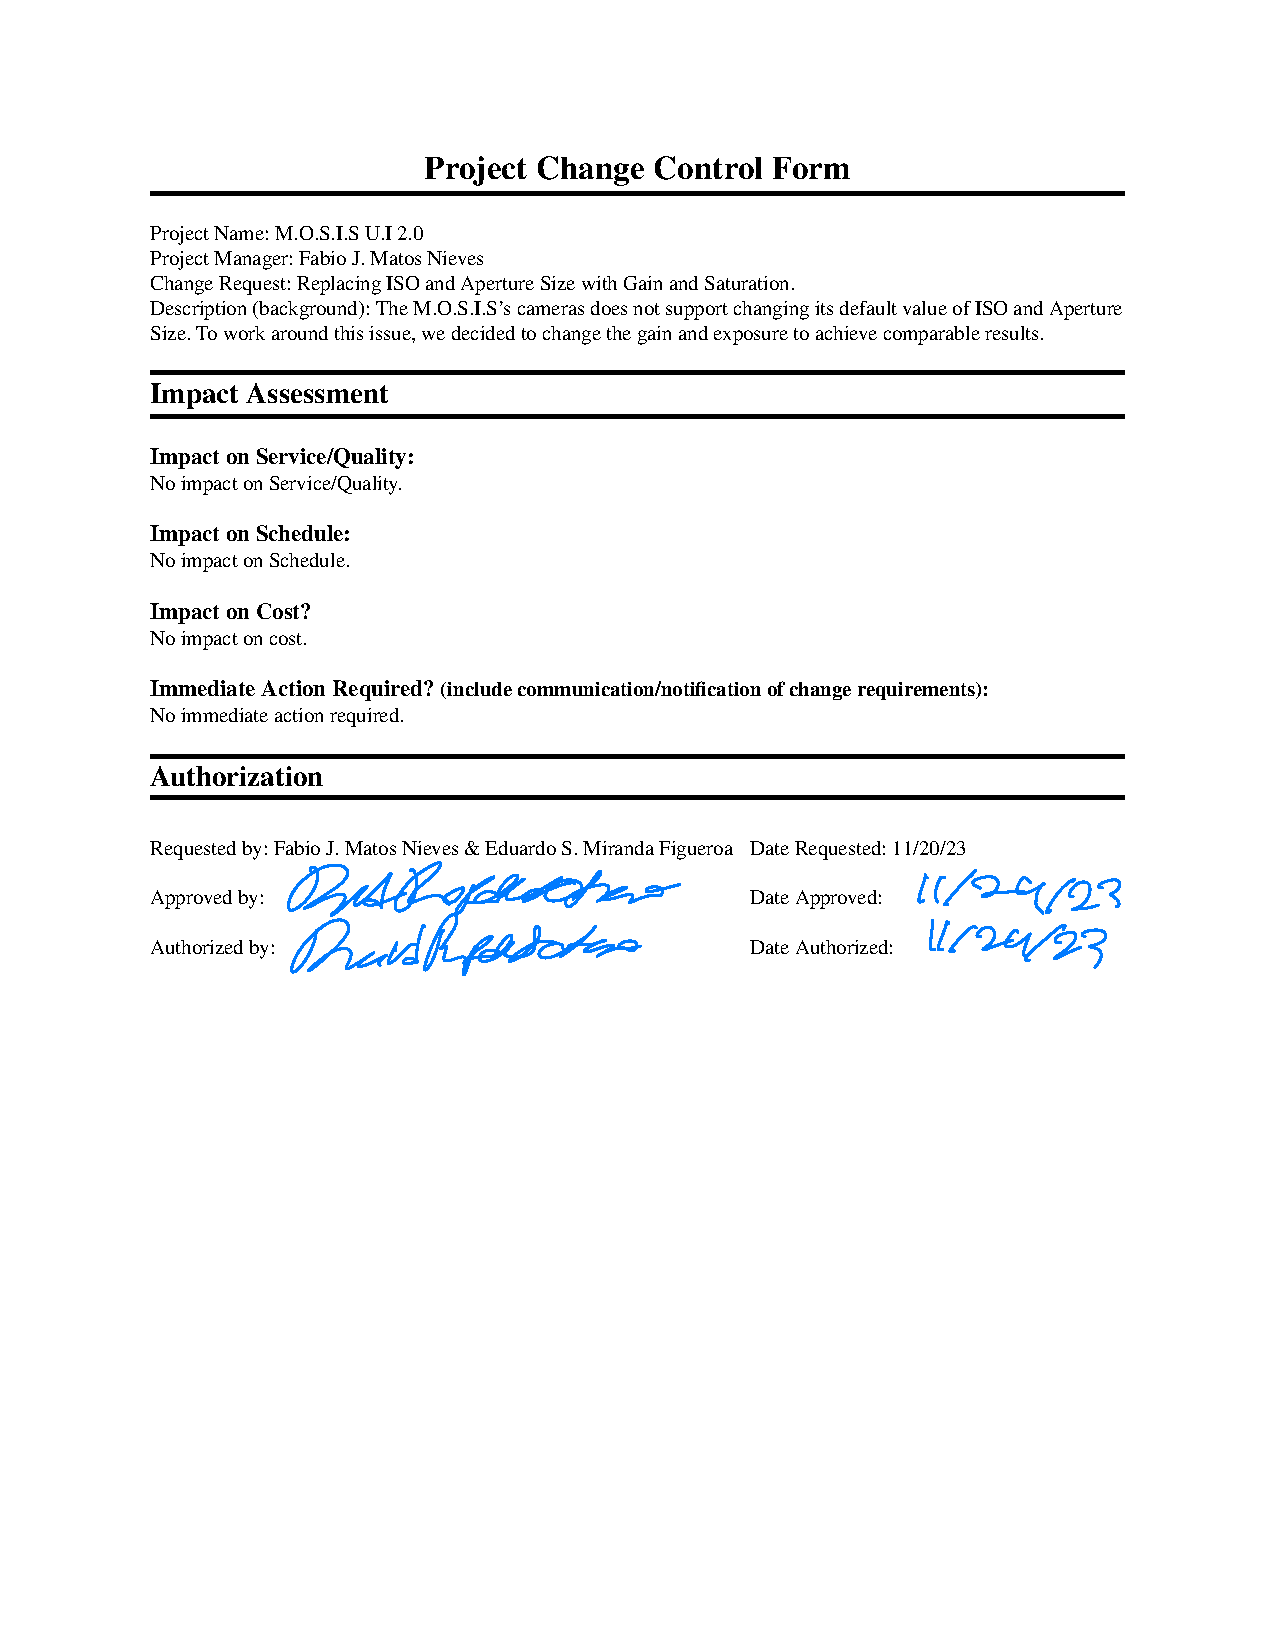
\includepdf[pages=1-10]{../Appendix/Requirements/Figures/M.O.S.I.S_Requirement_Change_Control_Form_.pdf}

\section{System Specifications (Fabio \& Eduardo)}
Front End (Fabio \& Eduardo):
\begin{itemize}
	\item 400x400 resolution, 24 FPS preview of each camera (left and right)
	\item Left and right camera preview on preview screen
	\item Display Temperature (Celsius), pH, Gauge Pressure (mbar) and Dissolved Oxygen (mg/L), current IP address and study status at the bottom of the preview screen
	\item Study status indicates if a study is in progress
	\item List to select study profile
	\item Navigation using on board buttons
	\item Safe emergency shutdown using a single button
	\item Initiate study capture using a single button
	\item Navigate study profile using two buttons
	\item Start study capture using a single button
	\item Stop currently executing study using a single button
	\item View study list menu using one button
	\item Cycle through ISO control, shutter speed control, aperture size control, white balance control, pH sensor calibration and dissolved oxygen sensor calibration menus with a single button
	\item ISO control menu allows to select from 100, 200, 400, 800, 1600, 3200, 6400 ISO values
	\item Aperture size control menu allows to select from f1.4, f/2.0, f/2.8, f/3.5 f/4.0, f/5.6, f/8.0, f/11.0, f16.0, f/22.0
	\item Shutter speed control menu 1/2000, 1/1000, 1/500, 1/250, 1/125, 1/60, 1/30, 1/15, 1/8, 1/4, 1/2, 1.0, 2.0, 4.0, 8.0, 15.0, 30.0
	\item White balance control allows values from 1,000 to 10,000
	\item pH sensor calibration menu allows values from 0 to 14 on low, mid and high point settings
	\item Dissolved oxygen calibration menu allows to calibrate single point and double point settings and allows to clear calibration settings
\end{itemize}
Back End (Eduardo):
\begin{itemize}
	\item Store shot id , shot type, ISO, shutter speed, white balance and white balance in one table
	\item Store media id, shot id, left media path, right media path, ISO 8601 date stamp, illumination type, temperature, dissolved oxygen, pH and pressure in one table
	\item Relate shot id to all media with that specific shot id
	\item Select all table related to a study using shot id
\end{itemize}
Hardware API (Fabio):
\begin{itemize}
	\item Document existing, transferable camera library functions
	\item Adapt camera functions to utilize database and folder structure schema
	\item Receive sensor data from UART port with a baud rate of 115200, 8 data bits and 1 stop bit
	\item Split sensor data string at the ampersand character
	\item Create a JSON file from the data and metadata
\end{itemize}
Folder Structure Generator (Eduardo):
\begin{itemize}
	\item Create folder based on Id, shot type, ISO 8601 date stamp, illumination type and camera settings
	\item Store all media files within the created folder
	\item Store JSON file with all data and metadata associated with the study in the same folder as the media files
	\item Identify media entry using shot id, ISO 8601 date stamp, illumination, ISO, shutter speed, aperture size and white balance
\end{itemize}
\section{Analysis of Alternatives (Fabio)}
\subsection{Front End}
In order to establish what alternatives we have to create our design, we first need clearly define what is the domain of our system. First, the hardware this system to be is going to used on is a underwater microscope used to capture the environmental conditions of the specimens to be studied \textit{in situ}, or on site. This microscope has two cameras, a left and a right camera used to later generate a stereoscopic image of the captured media. The microscope also has 4 on board sensors, temperature, pH, pressure and dissolved oxygen sensors used to capture the environmental conditions under the water. The microscope has a total of 8 buttons that serve as only way to interact with the device under the water and a 800x480 resolution display as its view into the real time operating system Raspberry Pi OS.\\
Now that the domain has been clearly established we can now discuss what alternatives we have at our disposal to create a user interface. There are 3 main ways to create a user interface on a computer:
\begin{enumerate}
	\item In the web browser or web based.
	\item A Native application.
	\item Using electron or React native, i.e Native Browser.
\end{enumerate}
Each one of these design alternatives have their advantages and disadvantages individually, but, in order to properly analyze their potential advantages and disadvantages, we first have to put it in the context of what the M.O.S.I.S microscope is.\\
At its core, the M.O.S.I.S microscope is a Raspberry Pi microcontroller with sensors and cameras attached to it that runs of a battery. Given that the Raspberry Pi is a single core, 1.8GHz ARM processor with 4GB of system memory using an SD Card for booting the Raspberry Pi OS which is a Debian Linux distribution specifically designed for use on the Raspberry Pi microcontroller.\cite{ltdRaspberryPiModel}\cite{DebianUniversalOperating} Given the hardware that the system-to-be is going to be running on is in term of computing resources, we could easily eliminate both web based and native browser alternatives right then and there since web browsers are large pieces of software that do not run particularly well on limited hardware. The web based architecture also has problems with accessing low level aspects of the system easily and with little overhead. This is due to the fact that a web browser is a completely sandboxes environment for code execution, meaning that a web based implementation would need to establish a client and server relationship to access hardware directly via the server. A web based implementation also suffers from being not particularly efficient in terms of CPU cycles and memory usage due to the sandboxed nature and having much more features than what is needed for our design. By extension, a native browser implementation would suffer a lot of the same drawbacks as a purely web based application. A native browser implementation is closer to the hardware since a native client is compiled to the target hardware and a web like environment is spawned inside the client. This kind of implementation accelerates deployment on many platforms, such as discord that has clients for Windows, Mac, IOS, Android, Linux and the browser only using a single main code base.\cite{Discord2023}  This advantage is of no benefit to this project since the M.O.S.I.S microscope is purpose built piece of hardware with a lot of software already written specifically for it and thus portability is not of any use in this case. A native browser implementation also suffers from being resource intensive, especially in the memory department, where a single instance of an application uses hundreds of megabytes of memory for a single application.\\
This leads us then to create a native application, but this then poses an interesting question, how do we make a native application? There are a plethora of options to use, .NET from Microsoft, Qt and GTK from Linux, or even newer libraries such as Iced from Rust and many more. In order to narrow down which alternatives work in our case, we again have to look at our domain. The Raspberry Pi peripheral access library is officially supported way to interact with the on board peripherals on the Raspberry Pi. The Raspberry Pi library only officially supports the Python programming language. There are wrappers or bindings for the Pi's library functions in other languages such as Rust, but they are not officially supported by the vendors of the Pi. Therefore, we are restricted building our system in the Python programming language.\\
Now that we have defined our domain and chosen programming language, now we have the task of selecting which UI library (or none) to use. Let us get of the way the option of not using a UI library up front. Given that by the end of the semester we have to give a prototype based on our design, allocating a large portion of our allotted development time into creating just the markup of the UI without the help of a library would be not only inadvisable but also delay the project to the point that a on time delivery would be impossible. Creating a new UI framework between a team of two in less than 3 months is simply impossible.\\
There are plenty of options of UI library bindings for Python: TKinter, PyQt, PyGTK, Kivy, PySimpleGUI and WxPython just to name a few. We can safely discard TKinter immediately because the current UI for the M.O.S.I.S microscope is written in TKinter and has a myriad of issues such as being undocumented, antiquated, buggy and slow. WxPython are binding for Python for the popular wxWidgets library in C++. It is well liked among developers of proprietary software since its ``modified version of LGPL explicitly allowing not distributing the sources of an application using the library even in the case of static linking.``\cite{WxWidgetsWxWidgets2023} However, due to the teams objections to having such a restrictive license, we have decided to not use wxWidgets. PySimpleGUI would be a valid option but, it only serves to simplify tools such as TKinter, Qt and WxPython and is not a UI library onto its own. Plus it is relatively new, from 2018, thus it is not as battle tested as other alternatives in the UI library landscape. Kivy is purely written in Python and is meant to be portable, for use in mobile applications. Due to concerns over performance of the Python programming language the team opted not to use Kivy. This now leads to the big two in the Linux ecosystem Qt and GTK with their associated Python bindings PyQt and PyGTK respectively.\\
GTK was initially released on April 14, 1998 and is the UI library used in all GNOME desktop applications and GNOME is the flagship desktop environment for the most widely used Linux distribution, Ubuntu.\cite{GNOME2023}\cite{Ubuntu2023} It is licensed under the GPL and currently is on version 4.10 and is still actively maintained. QT was released May 20, 1995 and is the UI library used in all KDE applications.\cite{QtSoftware2023} Most famously, KDE Plasma is the desktop environment used in the wildly successful Steam Deck.\cite{SteamDeck2023} Qt is licensed under LGPL, GPL and Qt Commercial License.\cite{QtLicensingQt} Both of the UI libraries meet our requirements of being open source and battle tested so the argument now comes down to developer experience.\\
GTK is an opinionated library, meaning that the GTK developers place heavy emphasis on having all GTK applications having a smaller look and feel. This is all well and good when making a consistent desktop environment in Linux but forces a certain design language across a wide range of applications. This would not be too much of a problem if it would be simple and straight forward to override the default styling and behaviors of the widgets that the GTK library offers but alas it is not simple. Overriding a simple button in GTK quickly devolves into several dozen lines of boilerplate code just to change the label of a button. Never mind doing this overriding on several dozen widgets, which quickly degrades the quality of the code base and reduces readability of the source code.\\
Qt allows for the individual widgets to have a customized style sheet, with CSS like syntax, in order to achieve the look and feel as desired. Qt also has much simpler syntax than GTK which allows for more rapid prototyping. Qt also provides Qt designer, a tool that allows the creating user interface mark up in a graphical interface. This is in stark contrast to GTK where the developer has to manually create the markup using XML. GTK is also criticized for having an unstable development cycle where there are major changes to the library rather frequently where as Qt has a much more stable development cycle. Given all this analysis we chose PyQt to be our UI library of choice going forward in this project.\\
\subsection{Database}
Now for the database, databases come in two main flavors, relational and non-relational databases. The M.O.S.I.S microscope only captures four fields, temperature, pH, pressure and dissolved oxygen using its onboard sensors, four field for camera configuration, two fields for study configuration, the time a metadata entry was captured and two fields for absolute paths for the captured media. This gives us a total thirteen total field to be captured related by a simple entry identifier. As a team, we realized that given the simple relationship  between the recorded fields, a relational database was the best choice given our use case.\\
As for what relational database engine to use, that requires to again look at the microscope's hardware limitations and project objectives. The Raspberry Pi only has 4GB of system memory and a single CPU core running at 1.8GHz, running off a battery, in an environment without internet that can quickly destroy the hardware. Most databases utilize a server to communicate with the database, MySQL, PostgreSQL, Microsoft SQL server, and MongoDB all utilize this client server relationship. This style of database works great for concurrent applications where hundreds if not thousands of requests to and from the database are made every second. The backup of these kinds of databases rely on mirroring the database on an off site backup on a regular basis. However, both of these advantages are null and void in our use case since the microscope will be in an environment without internet until the data is off loaded, utilized by users that do not know how to perform a database backup and that the hardware the database is limited, meaning that both space, CPU usage and memory use are a major concern. This leads us to a database engine called SQLite, a single threaded, synchronous relational database that stores itself in a file. It is the de facto standard in embedded, desktop and smartphone applications where a more sophisticated database alternative is unfeasible or impractical. As mentioned it stores itself in a file, making it simple to backup the database. It has four types for all data: text, integer, real and blob, meaning that the database engine can compile and compress the data much more efficiently. The single threaded nature of SQLite also lends it self well to the Raspberry Pi to conserve computing resources. As the name suggests SQLite uses SQL syntax meaning that any future maintainers of this project need not learn and exotic database query language to interact with it. Given how well SQLite meets the requirements for out use case we have chosen it to be our database going forward.
\section{System Architecture and Interfaces}
\subsection{Hardware Block Diagram}
\begin{figure}[H]
  \begin{center}
    \includesvg[inkscapelatex=false,width=0.95\textwidth]{../Appendix/System_Architecture_and_Interfaces/Hardware_Block_Diagram/Figures/hardware_block_diagram.svg}
  \caption{M.O.S.I.S Microscope Block Diagram}
  \end{center}
\end{figure}
\subsection{Hardware Interfaces Documentation (Given)}
\begin{figure}[H]
  \begin{center}
    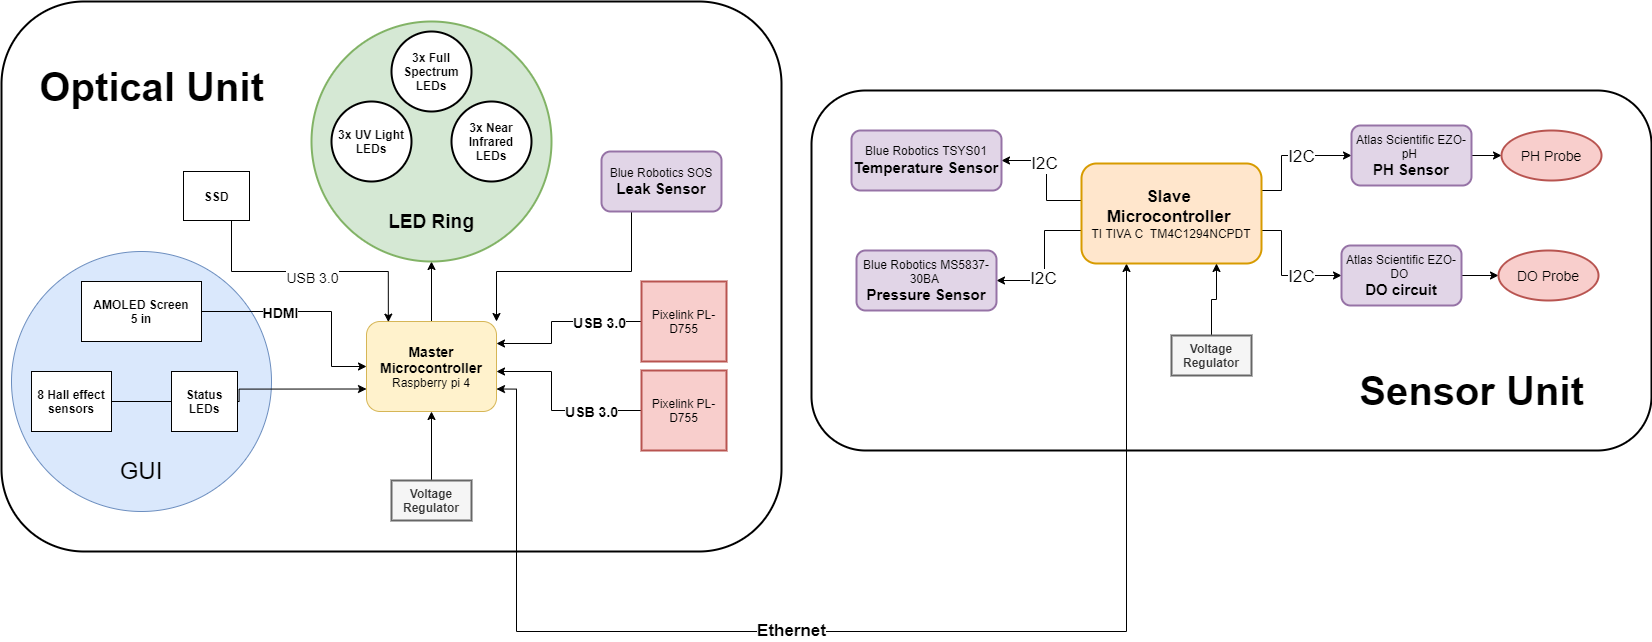
\includegraphics[width=0.95\textwidth]{../Appendix/System_Architecture_and_Interfaces/Hardware_Interfaces_Documentation/Figures/interfaces_diagram.png}
  \caption{M.O.S.I.S Interface Diagram}
  \end{center}
\end{figure}
\textbf{Note: All Diagrams from appendices E.3 to I are compliant to the UML 2.0 standard}
\subsection{Software Architecture}
\subsection{Software Interfaces}
M.O.S.I.S UI 2.0 has a total of three communication interfaces between the various peripherals:
\begin{enumerate}
\item UART Port
\item Camera SDK
\item UNIX File system
\end{enumerate}
The UART port is used to communicate with the sensor hub. The sensor hub provides methods to calibrate both pH and dissolved oxygen sensors and receive temperature, pH, pressure and dissolved oxygen data, in the form of a string, from the sensor hub sensors (See \ref{s:other_documentation} for detailed information on the sensor hub). The UART port on the sensor hub is configured with a baud rate of 115200 baud, 8 data bits, 1 stop bit and no parity bit on the port ``/dev/ttyAMA0'' on GPIO pins 14 and 15.\cite{UARTRaspberryPi} The camera SDK is the proprietary vendor software development kit by Pixelink used to communicate with both of the on board cameras.\cite{WhatFunctionsFeatures}. Finally, the UNIX file system is used to save, move, rename, read, write and delete the media files generated by the camera as well storing the SQLite database for the UI. The UNIX file system can be interacted directly by system calls, by shell abstractions such as cp, cd and mv or by the ``os'' or ``shutil'' packages in Python.\cite{SystemCallsUnix}\cite{UnixShellSummary}\cite{OsMiscellaneousOperating}\cite{ShutilHighlevelFile}

\section{Design Documentation}
\subsection{Design Justification (Eduardo)}
\subsubsection{Use Case Diagram}
Since this is a user facing application, the bulk of the use cases are attributed to the users. However, the reason why the application itself is responsible for performing diagnostics is to avoid an invalid state for the user interface to start. The use cases were derived from the requirements from the client and stakeholder.
\subsubsection{Class Diagram}
The U.I abstract class follows the PyQt6 module layout. The reason the U.I abstract class is dependent on application is that without an application there are no U.I elements to be rendered. The U.I abstract class having hide and show methods allows flexibility in designing the user interface, so that it allows all U.I menus and screens to be in a single PyQt6 widget window. Thus reducing the time between menus and screen spawning since they are already loaded into the application. As for why shot types and illumination types are enums is that one single can be present at any given time. The sensor abstract class has call and exit methods in a call command, since the sensor hub UART interface is designed to accept a call command to enter a sensor's subroutine and exit that subroutines when writing ``exit'' to the UART port. Finally the study profile is the internal representation of a JSON file loaded from the external host software.
\subsubsection{U.I Mockups}
The color scheme that we chose for the background is black with neon orange text and gray background with neon green text. The reason why the background colors for the U.I mockups are gray and black are because we utilized studies that show that the color black and gray looks darker underwater.\cite{AquaticSafetyGroup2021}\cite{FluoGreenMost2018} Likewise the same studies show that bright colors such as neon orange and neon green looks equally as bright underwater.\cite{AquaticSafetyGroup2021}\cite{FluoGreenMost2018} This insures that the researchers and divers have high contrast in environments with poor visibility.
\subsection{Hardware Schematics}
\begin{figure}[H]
  \begin{center}
    \includegraphics[width=0.95\textwidth]{../Appendix/Design_Documentation/Hardware_Detailed_Schematics/Figures/OCUSIS_Schematic_HD.png}
  \caption{M.O.S.I.S Hardware Schematics}
    \end{center}
\end{figure}
\newpage
\subsection{Firmware Flowcharts}
\begin{figure}[H]
	\begin{center}
		\resizebox{!}{0.8\textheight}{
			\import{../Appendix/Design_Documentation/Firmware_Flowcharts/Figures/}{get_snapshot_flowchart}
		}
	\end{center}
	\caption{M.O.S.I.S UI 2.0 Get Snapshot Flowchart}
\end{figure}
\subsection{Module Description}

\subsection{User Interface}
\subsection{Use Case Diagrams (Fabio)}
\begin{figure}[ht!]
	\resizebox{0.8\textwidth}{!}{
		\import{../Appendix/Design_Documentation/Use_Case_Diagram/Figures/}{use_case}
	}
	\caption{M.O.S.I.S UI 2.0 Use Case Diagram}
\end{figure}
\subsection{Class Diagrams}
\begin{figure}[ht!]
	\resizebox{\textwidth}{!}{
          \import{../Appendix/Design_Documentation/Class_Diagram/Figures/}{class_diagram}
	}
	\caption{M.O.S.I.S UI 2.0 Class Diagram}
\end{figure}
\subsection{Sequence Diagram}
\begin{figure}[ht!]
	\resizebox{\textwidth}{0.875\textheight}{
		\import{../Appendix/Design_Documentation/Sequence_Diagram/Figures/}{sequence}
	}
	\caption{M.O.S.I.S UI 2.0 Sequence Diagram}
\end{figure}
\subsection{Activity Diagram}
\begin{figure}[ht!]
	
    \includesvg[inkscapelatex=false,height=0.95\textheight]{../Appendix/Design_Documentation/Activity_Diagram/Figures/Activity_Diagram.svg}
	
	\caption{M.O.S.I.S UI 2.0 Activity Diagram}
\end{figure}

\subsection{ER Diagram}
\begin{center}
\begin{figure}[ht!]
  \resizebox{!}{0.8\textheight}{
   \import{../Appendix/Design_Documentation/ER_Diagram/Figures}{ER_Diagram.tex}
  }
%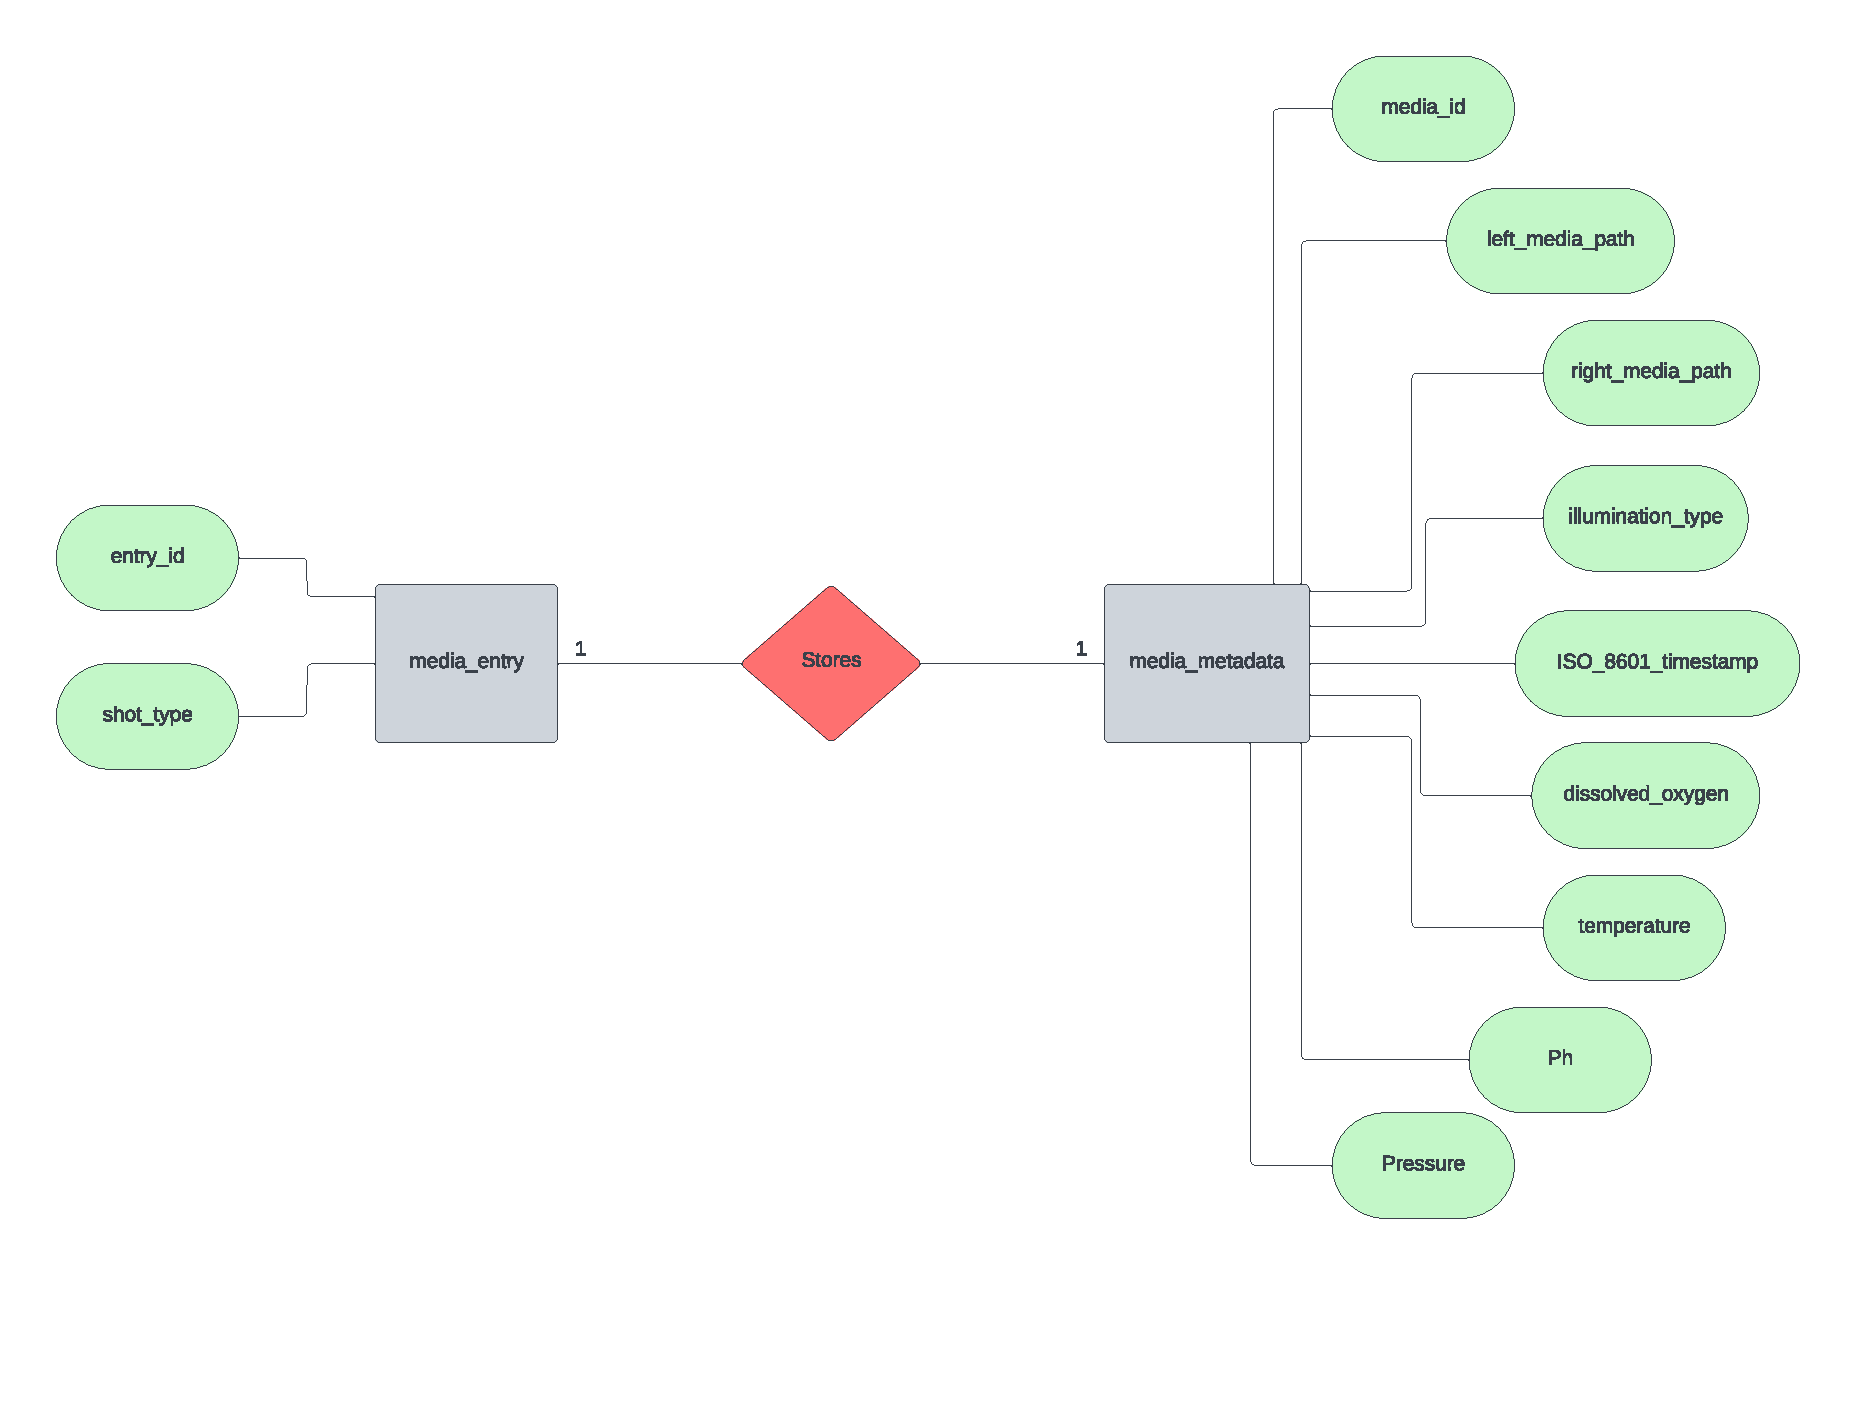
\includegraphics[page=1,width=\textwidth]{../Appendix/Design_Documentation/ER_Diagram/Figures/ER_Diagram_MOSIS.pdf}
  \caption{M.O.S.I.S UI 2.0 ER Diagram}
\end{figure}
\end{center}
\subsection{Other Documentation}
\section{Testing Plan (Eduardo)}
The Requirements to be tested are:
\begin{itemize}
    \item The system-to-be must present the left and right camera feeds to the user.
\end{itemize}
To test this requirement we will make sure that both feed are refreshing at 24 FPS and that the feed are at the specified 400 X 400 resolution.
\begin{itemize}
    \item The system-to-be must present temperature, Ph, dissolved oxygen, pressure, study status, and local IP address to the user.
\end{itemize}
To test this requirement we will verify that the sensors data presented are the same as the data received by the sensors and are updated every 2 seconds.
\begin{itemize}
    \item The system-to-be must have the means to switch between different study profiles
\end{itemize}
To test this requirement we will add functionality to the on board buttons that allows the user to switch between different study profiles.
\begin{itemize}
    \item The system-to-be must control the lighting on the microscope cameras according to the study profile.
\end{itemize}
To test this requirement we will verify that the lighting on the study data is the one according to the study profile.
\begin{itemize}
    \item The system-to-be must control the shot type on the microscope cameras according to the study profile.
\end{itemize}
To test this requirement we will verify that the shot type on the study data is the one according to the study profile.
\begin{itemize}
    \item The system-to-be must control the ISO of the microscope cameras.
\end{itemize}
To test this requirement we will verify that the ISO on the study data is the one according to the study profile.
\begin{itemize}
    \item The system-to-be must control the aperture size of the microscope cameras.
\end{itemize}
To test this requirement we will verify that the aperture size on the study data is the one according to the study profile.
\begin{itemize}
    \item The system-to-be must control the shutter speed of the microscope cameras.
\end{itemize}
To test this requirement we will verify that the shutter speed on the study data is the one according to the study profile.
\begin{itemize}
    \item The system-to-be must control the white balance of the microscope cameras.
\end{itemize}
To test this requirement we will verify that the white balance on the study data is the one according to the study profile.
\begin{itemize}
    \item The system-to-be must call the calibration functions of the microscope sensors.
\end{itemize}
To test this requirement when calling the calibration functions of the microscope sensors we will check that the sensors are being calibrated as per the user.
\begin{itemize}
    \item The system-to-be must have a database that stores:
    \begin{itemize}
        \item Left Camera Media
        \item Right Camera Media
        \item Shot type
        \item ISO 8601 Date Stamp (yyyy-MM-ddTHH:mm:ss.zzz)
        \item Temperature
        \item Ph
        \item Pressure
        \item Dissolved Oxygen
        \item Illumination Type
        \item ISO
        \item Aperture Size
        \item Shutter Speed
        \item White Balance
    \end{itemize}
\end{itemize}
To test this requirement we will check the data on the study completely matches the data on the database.
\begin{itemize}
    \item The system-to-be must store the captured data into a browsable format.
\end{itemize}
To test this requirement we will verify on the host computer that the data stored is able to be browsed without difficulty.
\begin{itemize}
    \item The system-to-be must use the on board buttons to control the functions of the microscope.
\end{itemize}
To test this requirement we will verify that each on board button is performing their intended function.
\begin{itemize}
   \item The system-to-be must present the feed from left and right cameras, each at 24FPS and a downscaled 400x400 resolution.
\end{itemize}
To test this requirement we will make sure that both feed are refreshing at 24 FPS and that the feed are at the specified 400 X 400 resolution.
\begin{itemize}
    \item The system-to-be must present: temperature, Ph, pressure, dissolved oxygen, study status, ISO, aperture size and shutter speed, white balance and IP address.
\end{itemize}
To test this requirement we will verify that the sensors data presented are the same as the data received by the sensors and are updated every 2 seconds.
\begin{itemize}
    \item The system-to-be must update temperature, Ph, pressure, dissolved oxygen and local IP address, study status, every two seconds due to the existing UART implementation.
\end{itemize}
To test this requirement we will verify that the updated data shown are the correct data from the existing UART implementation.
\begin{itemize}
    \item The system-to-be lighting enumeration contains:
    \begin{itemize}
        \item None
        \item Infrared
        \item Ultraviolet
        \item Visible Spectrum
    \end{itemize}
\end{itemize}
To test this requirement we will verify that the function for lightning enumeration includes: none, infrared, ultraviolet and visible spectrum. The cameras will also have the capability to change the lighting as per the user.
\begin{itemize}
    \item The system-to-be shot type enumeration contains:
	      \begin{itemize}
		      \item Single
		      \item Burst
		      \item Telescopic
		      \item Time Lapse
		      \item Video
	      \end{itemize}
\end{itemize}
To test this requirement we will verify that the function for lightning enumeration includes: single, burst, telescopic, time lapse and video. The cameras will also have the capability to change the shot type as per the user.
\begin{itemize}
    \item The system-to-be must initiate a capture with a single button.
\end{itemize}
To test this requirement we will verify that the system-to-be starts capture with the use of only one button.
\begin{itemize}
    \item The system-to-be must shutdown the operating system safely with a single button.
\end{itemize}
To test this requirement we will verify that the system-to-be starts shutdown procedure safely with the use of only one button.
\begin{itemize}
    \item The system-to-be must stop capture with a single button.
\end{itemize}
To test this requirement we will verify that the system-to-be stop capture with the use of only one button.
\begin{itemize}
   \item The system-to-be must be able to navigate through the study profiles using only two buttons.
\end{itemize}
To test this requirement we will verify that the system-to-be is able to navigate through the study profiles using only two buttons.
\begin{itemize}
	\item The system-to-be must show the currently loaded study profiles using a single button.
\end{itemize}
\begin{itemize}
    \item The system-to-be must store all files related to a single study entry in a single directory.
\end{itemize}
\begin{itemize}
    \item The system-to-be must store a JSON file with all data and metadata from the study entry along in the same directory as the study entry.
\end{itemize}
\begin{itemize}
    \item The system-to-be must control the focus of the cameras one stepper motor step at a time using two buttons.
\end{itemize}
\begin{itemize}
    \item The system-to-be must control the ISO of the cameras using two buttons.
\end{itemize}
\begin{itemize}
    \item The system-to-be must show all available camera ISO using a single button.
\end{itemize}
\begin{itemize}
    \item The system-to-be must control the aperture size of the cameras using two buttons.
\end{itemize}
\begin{itemize}
    \item The system-to-be must show all available aperture sizes using a single button.
\end{itemize}
\begin{itemize}
    \item The system-to-be must control the shutter speed of the cameras using two buttons.
\end{itemize}
\begin{itemize}
    \item The system-to-be must show all available shutter speeds using a single button.
\end{itemize}
\begin{itemize}
    \item The system-to-be must control the white balance of the cameras using two buttons.
\end{itemize}
\begin{itemize}
    \item The system-to-be must show all available white balance using a single button.
\end{itemize}
\section{Economic Analysis (Eduardo)}
\section{Task Progress and Gantt Chart (Eduardo)}
\end{document}
